\documentclass[a4paper,12pt]{report}

\nocite{*}

\newcommand{\nameInitial}{
    \textcolor{black}{G. Allen}  %change colour to black and enter your initial and surname
}
\newcommand{\nameFull}{
    \textcolor{black}{Gary Allen} %change colour to black and enter your firstname and surname
}
\newcommand{\stNumber}{
    \textcolor{black}{23905093} %change to black and enter your student number 
}
\newcommand{\myDate}{\textcolor{black}{\today} %change colour and if you want to date.
}
\newcommand{\signature}{frontmatter/fig/Signature}   %Upload your signature as "frontmatter/fig/Signature.png"


%%%%%%%%%%%%%%%%%%%%%%%%%%%%%%%%%%%%%%%%%%%%%%%%%%%%%%%%%%%%%%%%%
%From here you can ignore up to \begin{document} (line 107)
%%%%%%%%%%%%%%%%%%%%%%%%%%%%%%%%%%%%%%%%%%%%%%%%%%%%%%%%%%%%%%%%%
% Page layout
\usepackage[left=2.2cm,right=2.2cm,top=2.2cm,bottom=2.2cm]{geometry}
% Figures
\usepackage[margin=\the\parindent,small,bf,sf]{caption}
\usepackage{graphicx}
\usepackage{pdfpages}
\setlength{\abovecaptionskip}{7.5pt}  % spacing above and below captions
\newcommand*{\WaterMark}[2][0.2\paperwidth]{\AddToShipoutPicture*{\AtTextCenter{\parbox[c]{0pt}{\makebox[0pt][c]{\includegraphics[width=#1]{#2}}}}}}
\usepackage{subcaption}
% Font and text
\usepackage[afrikaans,english]{babel}
\usepackage{microtype}
\usepackage{setspace}
\usepackage{lmodern}
\newcommand{\myemph}[1]{{\sffamily\bfseries#1}}
\sloppy
\onehalfspacing
\usepackage{siunitx}
\usepackage{lipsum}
% Headings
\usepackage[raggedright,sf,bf]{titlesec}
\titlelabel{\thetitle.\ }
\titleformat{\chapter}[display]{\huge\bfseries\sffamily}{\chaptertitlename\ \thechapter}{15pt}{\raggedright}
% \titleformat{\chapter}[display]{\centering\huge\bfseries\sffamily}{\chaptertitlename\ \thechapter:}{15pt}{}
\titlespacing*{\chapter}{0pt}{0pt}{10pt}  % remove spacing before chapter headings
% Table of contents
\makeatletter
\let\originall@chapter\l@chapter
\def\l@chapter#1#2{\originall@chapter{{\sffamily #1}}{#2}}
\makeatother
\let \savenumberline \numberline
\def \numberline#1{\savenumberline{#1.}}
% Mathematics
\usepackage[cmex10]{amsmath}
\usepackage{amssymb}
\usepackage{cancel}
\DeclareMathOperator*{\argmax}{arg\,max}
\newcommand{\T}{^\textrm{T}}
\newcommand{\tr}{\textrm{tr}}
\renewcommand{\vec}[1]{\boldsymbol{\mathbf{#1}}}
\newcommand{\defeq}{\triangleq}
% Tables
\usepackage{booktabs}
\usepackage{tabularx}
\usepackage{multirow}
\newcommand{\mytable}{
    \centering
    \small
    \renewcommand{\arraystretch}{1.2}
    }
\renewcommand{\tabularxcolumn}[1]{m{#1}}
\newcolumntype{C}{>{\centering\arraybackslash}X}
\newcolumntype{L}{>{\raggedright\arraybackslash}X}
% Header and footer
\usepackage{fancyhdr}
\pagestyle{fancy}
\fancyhf{}
\renewcommand{\sectionmark}[1]{\markright{\normalsize \thesection.\ #1}}
\fancyhead[C]{\nouppercase{\textit{\rightmark}}}
\fancyhead[RO]{\thepage}
% \fancyhead[LE]{\thepage}  % double-sided printing
\fancyfoot{}
\setlength\headheight{14.5pt}
\renewcommand{\headrulewidth}{0pt}
\fancypagestyle{plain}{\fancyhead{}
                       \renewcommand{\headrulewidth}{0pt}
                       \fancyfoot[C]{\thepage}}
% Pseudo-code
\usepackage{algorithm}  % should go before \usepackage{hyperref}
% Table of contents and hyperlinks
\usepackage{hyperref}
\hypersetup{colorlinks=true,linktoc=all,citecolor=black,linkcolor=black}
\usepackage[nottoc]{tocbibind}
% Pseudo-code
\usepackage{algpseudocode}  % should go after \usepackage{hyperref}
\renewcommand{\thealgorithm}{\arabic{chapter}.\arabic{algorithm}} 
\captionsetup[algorithm]{labelfont={bf,sf},font=small,labelsep=colon}
% Bibliography
\usepackage{cite}  % automatically reorder inline citations
\bibliographystyle{IEEEtran}
% Fix titlesec issue
\usepackage{etoolbox}
\makeatletter
\patchcmd{\ttlh@hang}{\parindent\z@}{\parindent\z@\leavevmode}{}{}
\patchcmd{\ttlh@hang}{\noindent}{}{}{}
\makeatother
 \usepackage[normalem]{ulem}
%%%%%%%%%%%%%%%%%%%%%%%%%%%%%%%%%%%%%%%%%%%%%%%%%%%%%%%%%%%%%%%%%
% Ignore up to here. 
%%%%%%%%%%%%%%%%%%%%%%%%%%%%%%%%%%%%%%%%%%%%%%%%%%%%%%%%%%%%%%%%%

\begin{document}

% Front matter
\graphicspath{{frontmatter/fig/}}
\pagenumbering{Alph}

\begin{titlepage}
\begin{center}


\includegraphics[width=8cm]{frontmatter/fig/SU_logo_RGB_without_slogan.pdf}

\vfill

{\sffamily \bfseries \huge E344 Assignment 1 \par}

\vfill

{\large {\Large \nameFull} \\ \stNumber \par}

\vfill

\vfill

{Report submitted in partial fulfilment of the requirements of the module \\
Design (E) 344 for the degree Baccalaureus in Engineering in the Department of
Electrical and Electronic Engineering at Stellenbosch University. \par}

\vfill

%{\large {Supervisor}: Dr L. Skywalker} %\\
% Department of Electrical and Electronic Engineering \par}

\vfill

{\Large \myDate}
\end{center}
\end{titlepage}

\pagenumbering{roman}
\graphicspath{{frontmatter/figures/}}
\newpage
\pagestyle{plain}
\addcontentsline{toc}{chapter}{Declaration}
\makeatletter\@mkboth{}{Declaration}\makeatother

\centerline{
\includegraphics[width=8cm]{SU_horizontal_RGB.pdf}}
\vspace*{-10pt}

\section*{\centering Plagiaatverklaring / \textit{Plagiarism Declaration}}

\vspace*{5pt}

\begin{enumerate}
    \item Plagiaat is die oorneem en gebruik van die idees, materiaal en ander intellektuele eiendom van ander persone asof dit jou eie werk is.\\
    \textit{Plagiarism is the use of ideas, material and other intellectual property of another's work
        and to present is as my own.}
    
    \item Ek erken dat die pleeg van plagiaat 'n strafbare oortreding is aangesien dit 'n vorm van diefstal is.\\
    \textit{I agree that plagiarism is a punishable offence because it constitutes theft.}
    
    \item Ek verstaan ook dat direkte vertalings plagiaat is. \\
    \textit{I also understand that direct translations are plagiarism.}
    
    \item Dienooreenkomstig is alle aanhalings en bydraes vanuit enige bron (ingesluit die internet) volledig verwys (erken). Ek erken dat die woordelikse aanhaal van teks sonder aanhalingstekens (selfs al word die bron volledig erken) plagiaat is. \\
    \textit{Accordingly all quotations and contributions from any source whatsoever (including the internet) have been cited fully. I understand that the reproduction of text without quotation marks (even when the source is cited) is plagiarism}
    
    \item Ek verklaar dat die werk in hierdie skryfstuk vervat, behalwe waar anders aangedui, my eie oorspronklike werk is en dat ek dit nie vantevore in die geheel of gedeeltelik ingehandig het vir bepunting in hierdie module/werkstuk of 'n ander module/werkstuk~nie. \\
    \textit{I declare that the work contained in this assignment, except where otherwise stated, is my original work and that I have not previously (in its entirety or in part) submitted it for grading in this module/assignment or another module/assignment.}
\end{enumerate}

\vfill

\noindent \begin{tabularx}{1.0\linewidth}{|L|L|}
    \hline
    \hspace{2cm} \large{\stNumber}& \vspace{4mm}\hspace{2cm} \includegraphics[height=1.5cm]{\signature}\\

    \vspace{0mm}{Studentenommer / \textit{Student number}} & \vspace{0mm} {Handtekening / \textit{Signature}} \\
    \hline
    \vspace{1mm}  \hspace{2cm} \large{\nameInitial} & \vspace{1mm} \hspace{2cm} \large{\myDate }\\
    \vspace{1mm} {Voorletters en van / \textit{Initials and surname}} & \vspace{1mm} {Datum / \textit{Date}} \\
    \hline
\end{tabularx}

\vspace{15pt}




\tableofcontents
\listoffigures
\listoftables
\chapter*{Nomenclature\markboth{}{Nomenclature }}
\addcontentsline{toc}{chapter}{Nomenclature}

% \vspace*{-3mm}
\subsubsection*{Variables and functions}
\begingroup
\renewcommand{\arraystretch}{1.2}
\renewcommand{\tabularxcolumn}[1]{p{#1}}
\begin{tabularx}{\textwidth}{@{}p{2.5cm}L}
    $V_{ss}$            & Voltage positive.                     \\
    $V_{dd}$            & Voltage negative.                     \\
\end{tabularx}
\endgroup


%\newpage
\subsubsection*{Acronyms and abbreviations}


\begingroup
\renewcommand{\arraystretch}{1.2}
\begin{tabular}{@{}p{2.5cm} l}
    CMRR                & Common Mode Rejection Ratio           \\
    RC                  & Resistor-Capacitor                    \\
    PWM                 & Pulse Width Modulation                \\
    LPF                 & Low Pass Filter                       \\
    HPF                 & High Pass Filter                      \\
    TTL                 & Transistor-Transistor Logic           \\
    MCU                 & Microcontroller Unit                  \\
\end{tabular}
\endgroup

\newpage
\pagenumbering{arabic}

% Contents
%\chapter*{Example chapter - remove}\label{chap:Example}

You can remove this chapter by deleteting the ``\texttt{\textbackslash include\{Chapter0\}}'' line in the \texttt{e344\_A1\_report.tex} file.  

\textcolor{red}{The document you submit must not have ANY red text in - the text in red in this template is for information only}. 
Introduce the reader to what you want to present in this chapter. 
Think carefully of what you want to convey. You want the reader (e.g. another student) to understand the main concepts -- they need to understand enough to safely and efficiently \textbf{use} and \textbf{design for} a chassis car, but abstract enough to not get caught up in the minutiae of electrons. The person assessing your report will consider whether you have demonstrated that you were able to find, integrate (absorb), and effectively convey knowledge on this topic.   So, write a short summary of information you gathered from literature (papers, web sites, datasheets). Include any references to literature you feel is needed. Be sure to cite all the references, which you can add in the \texttt{References.bib} file, using the \texttt{\textbackslash\{cite\}} command.\\

\noindent Some examples of how to cite (all of these have been added in the  \texttt{References.bib} file): 
It was stated by \cite{Booysen:2013} that ... . Subsequently, he changed his mind and said in  \cite{Gerber:2019} that ... .
While \cite{WebsiteOpAmp} claims it to be ... .
Figure \ref{fig:someName} shows a figure, which could paint a thousand words (if it does not, rather use words)! Table \ref{tab:PVresults} could capture some of your datasheet and/or measured results.

\begin{figure}[!htb]
\centering
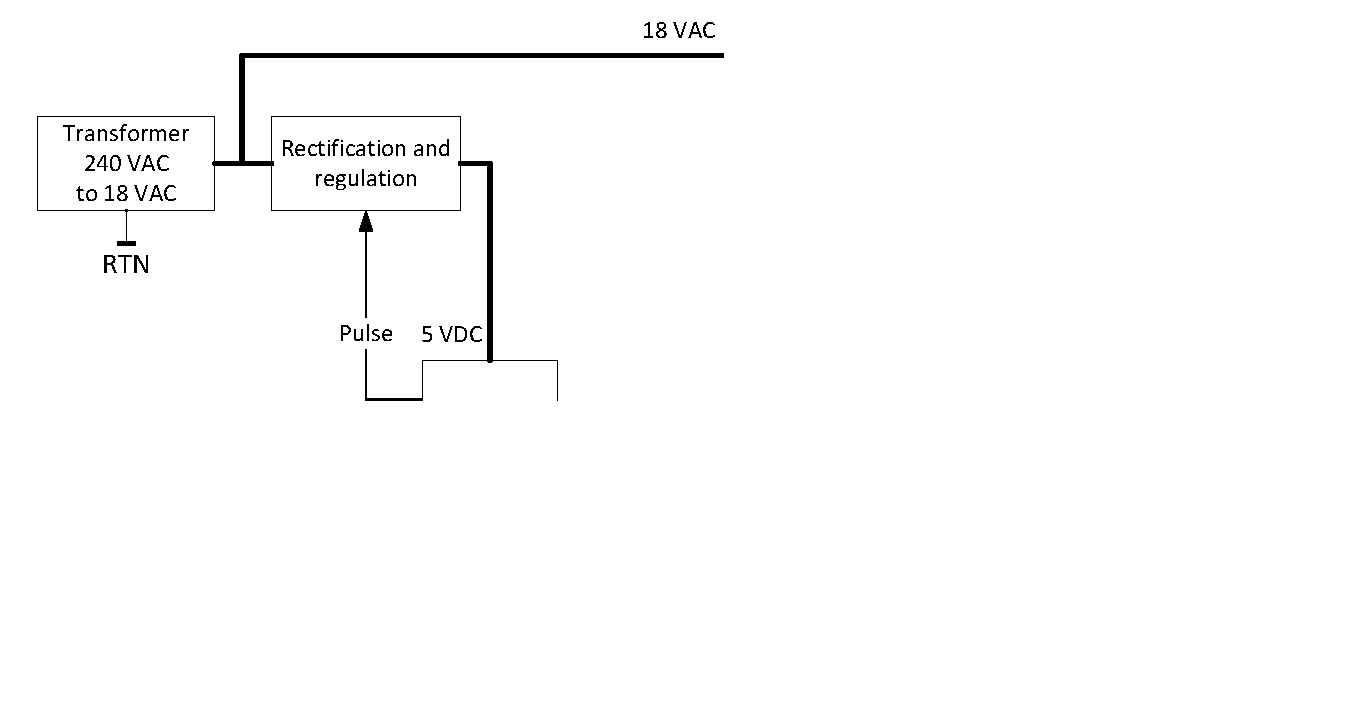
\includegraphics[width=0.5\linewidth]{Figures/PowerSystemDiagram.pdf}
\caption[This is my caption, make me descriptive!]{This is my caption, make me descriptive! And cite if you borrow figures \cite{WebsiteOpAmp}.}
\label{fig:someName}
\end{figure}

\begin{table}[!htb]
        \centering
        \footnotesize
        \caption{Example of a simple table.}
         \begin{tabular}{lrrrr}
          \toprule
             & $V_{OC}$ & $I_{CC}$ & $V_{pmax}$ \\
             &  [V]  & [A] & [V]\\
          \midrule
          Theroretical per cell & 1.0      & 1.0 & 1.0 \\
          Datasheet  per module &  1.0      & 1.0 & 1.0 \\
          Measured dark  1.0      & 1.0 & 1.0 \\
          Measured upside-down  1.0      & 1.0 & 1.0 \\
          Measured oblique  1.0      & 1.0 & 1.0 \\
          Measured facing  1.0      & 1.0 & 1.0 \\
          \bottomrule
        \end{tabular}
     \label{tab:PVresults}
\end{table}


\chapter{Literature survey}\label{chap:Lit}

Introduce the reader to \textbf{what you want to present} in this chapter (i.e.\ what are you trying to achieve by initiating this communication?).
Try to put yourself in the readers' shoes - what would you \sout{like} need to see to be convinced that the author (1) knew what they were doing and understood what they had to do (2) properly designed for the requirements, (3) simulation-tested their design, and (4) correctly and critically assessed the outcome. 

Include any references to literature you feel is needed. 
In this section, you put a very short summary of information you gathered from literature (papers, web sites, datasheets) that you used to do the design. Be sure to cite the references, which you can add in the \texttt{References.bib} file. 

\section{Operational amplifiers}\label{sec:opamps}

\subsubsection{Operational amplifiers: limitations and considerations}\label{sec:opamps_limits}

\subsubsection{Operational amplifier configurations}\label{sec:opamps_configs}


\section{Current sensing}\label{sec:cursens}

















\chapter{Detail design}\label{ch:detail_design}
%**********************************************
The following process details the design and calculations for the current sensor circuit. It provides insight into
what decisions were made, as well as the justifications behind them.

\section{Current sensor}\label{sec:current_sensor_design}
\subsubsection{Configuration}\label{sec:current_sensor_config}

The differential amplifier configuration will be used for this project for the following reasons:
\begin{itemize}
  \item The configuration is specifically designed to reject common-mode noise, which the non-inverting amp suffers from.
  \item Only 1 op-amp is needed.
  \item The design is relatively simple compared to the instrumentation amplifier.
\end{itemize}

However, a modified version with two extra capacitors will be used. Two capacitors will be added in parallel with $R_f$ and $R_g$ called $C_f$ and $C_g$ respectively. It is important that these capacitors have the same
value in order to preserve CMRR \cite{WebsiteOpAmpConfigurations}. It is likely, however, that one of these will be dominant due to differing resistor values, and therefore this design will only consider the filter to be first-order.
This is acceptable, however, due to the amplifier's noise-rejecting capabilities.

\subsubsection{Gain and Cutoff}\label{sec:current_sensor_circuit}
Before calculating component values, both the cutoff frequency of the RC filter, and the DC gain of the amplifier, need to be determined. The gain of the amplifier should be determined
such that, when the maximum current flows through the sense resistor, the maximum voltage is output.

First, the maximum current of the motor should be measured. This can be done by connecting the motor to a power supply (through an ammeter), stalling the motor, and reading the output current.
With a supply voltage of 6.4 V connected, the motor for this project read 740 mA, however different motors may read between 1 and 1.5 A. The average running current, however, is between 200 mA
and 300 mA. A value of $I_{max} = 1 A$ will therefore be chosen to allow for more headroom and a slightly lower gain.
Since a sense resistor of $\SI{10}{\milli\ohm}$ is to be used, the maximum voltage through this resistor will therefore be 8 mV. A gain of $\frac{3 V}{10 mV} = 300$ is therefore chosen.
Although this voltage level is small, it is expected, given that the resistance value is so small. It is also desirable, as it shows that the circuit is not "stealing" too much power from the motor itself.

The cutoff frequency $f_H$ should be selected such that the slew rate requirements are not affected, while still adequately filtering a 1 kHz noise signal. In order for the noise requirement
to be satisfied, the input signal must be attenuated by $20 \log{\frac{300 * 10 mV}{250 mV}} \approx 22 dB$. This means the cutoff should be around 100 Hz (a decade below 1 kHz).
Since the specification requires a change from 0.1 to $3 \times 0.9 = 2.7 V$ in less than 100 ms, the output should be capable of oscillating at $\frac{1}{50 ms} = 20 Hz$, which is below the designed cutoff.

Since input current of the circuit needs to be limited below 150 uA, high resistor values should be chosen:
\begin{itemize}
  \item Assuming $i_n = 0$, choose $\frac{V_{out(max)}}{R_1 + R_f} << 150 uA \therefore R_1 + R_f >> \SI{20}{\kilo\ohm}$. Choose $R_f = \SI{100}{\kilo\ohm}$.
  \item $G = \frac{R_f}{R_1} = 300 \therefore R_1 = \SI{330}{\ohm}$
  \item Choose $R_2 = R_1 = \SI{330}{\ohm}$ and $R_g = R_f = \SI{100}{\kilo\ohm}$ for differential symmetry.
  \item Since $R_{eq}$ of $C_f$ is $R_f$ and of $C_g$ is $R_g || R_2$, it is clear that $C_f$ is dominant, $\therefore C_f = \frac{1}{2 \pi \cdot R_f \cdot 100 Hz} \approx 15 nF$. Also set $C_g = 15nF$ for symmetry.
        It should be noted, however, that this technique (using time constants) is not always valid - especially in complex circuits such as these - and so these results should be checked using simulations.
\end{itemize}

\subsubsection{Circuit diagram}\label{sec:current_sensor_circuit}
The following figure details the final circuit design for the sensor and amplifier system.

\begin{figure}[h!]
  \centering
  \includegraphics[width=.8\linewidth]{Figures/Circuit}
  \captionof{figure}{Circuit diagram of final configuration}  
  \label{fig:circuit-diagram}
\end{figure}

A single 5 V supply will be used. Although there are benefits to a dual rail supply, that would prove impractical in the context of the larger system.

\pagebreak

\chapter{Results}\label{ch:results}

After running initial simulations, it was clear that the constant assumed in the design stage for the dominant capacitor $C_f$ was too high. The capacitor value was then experimentally
increased until a satisfactory response which was reasonably below 250 mV (10-20\%) was obtained. This section details the rest of the results of these simulations.

\begin{figure}[h!]
   \centering
   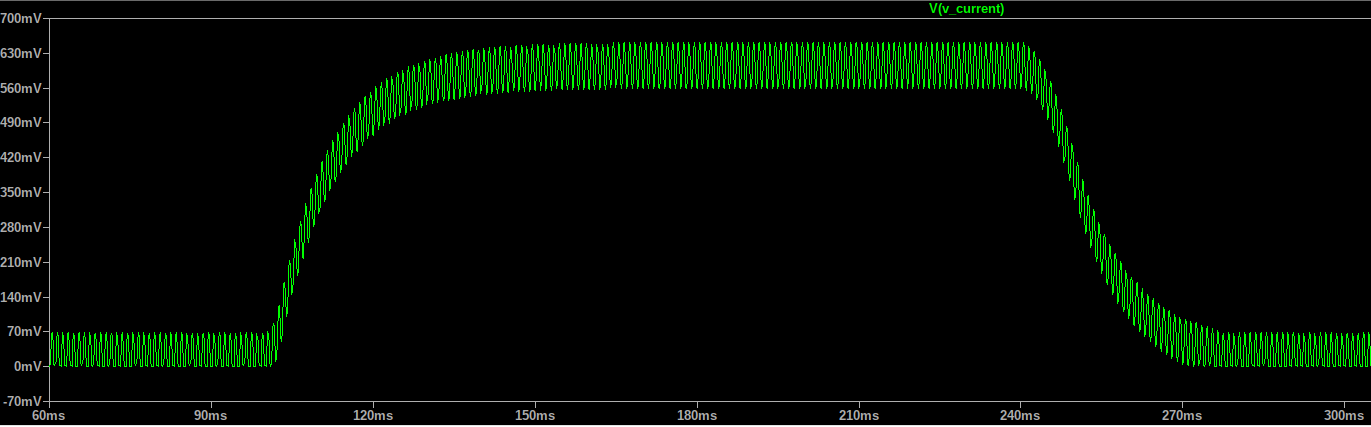
\includegraphics[width=.6\linewidth]{Figures/simulation_response}
   \captionof{figure}{Amplifier output in response to step input}
   \label{fig:simulation response}
\end{figure}

\begin{figure}[h!]
   \centering
   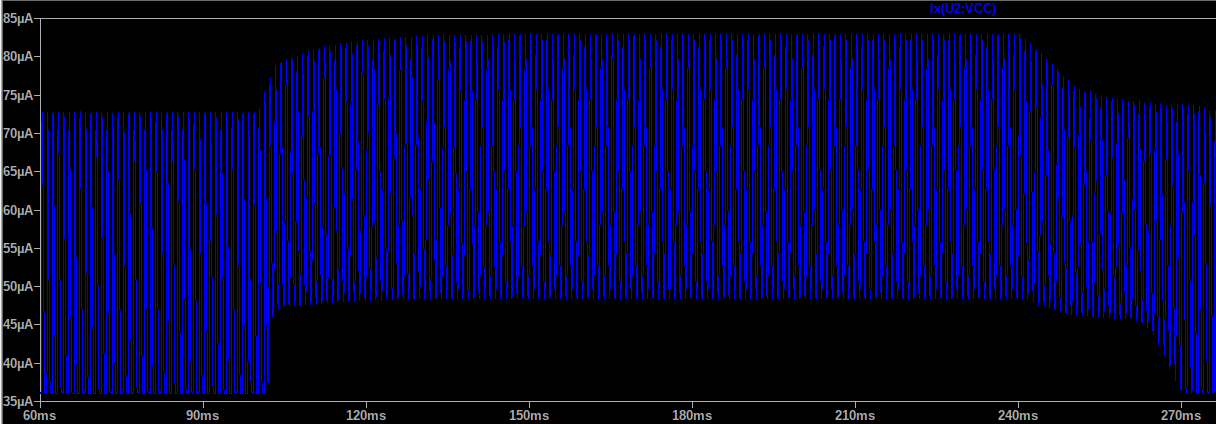
\includegraphics[width=.5\linewidth]{Figures/simulation_current}
   \captionof{figure}{Current draw of op-amp}
   \label{fig:simulation_current}
\end{figure}

As can be seen, all specifications were adhered to:
\begin{itemize}
   \item The noise level at idle is well below the 250 mV requirement.
   \item The step response input changes 20-25 ms, which is below the 100 ms requirement.
   \item The power draw of the circuit (as measure at the positive terminal of the op-amp) is less than 85 uA, which is much less than the specified 150 uA.
\end{itemize}

Lastly, the input simulation parameters were modified during testing to analyze the various output voltages for different input currents. For input currents of 400mA, 500mA, 800mA and 1A,
the output voltages were 1.22V, 1.52, 2.43 and 3.024 V respectively. This matches perfectly with the initial design.
\chapter{Physical implementation}\label{ch:implementation}

\section{Current sensor}\label{sec:current_sensor_physical}

The implementation of the circuit was different in two ways compared to the original design:
\begin{itemize}
   \item \SI{120}{\kilo\ohm} resistors were used instead of \SI{100}{\kilo\ohm}, as they were easier to obtain, and would only result in a
         slightly larger gain and lower cutoff.
   \item The amplifier circuit was powered with regulated \SI{3.3}{V}. This was done to protect the ESP's input pins by saturating the output
         when it would have been too large.
\end{itemize}

\begin{figure}[!htb]
  \centering
  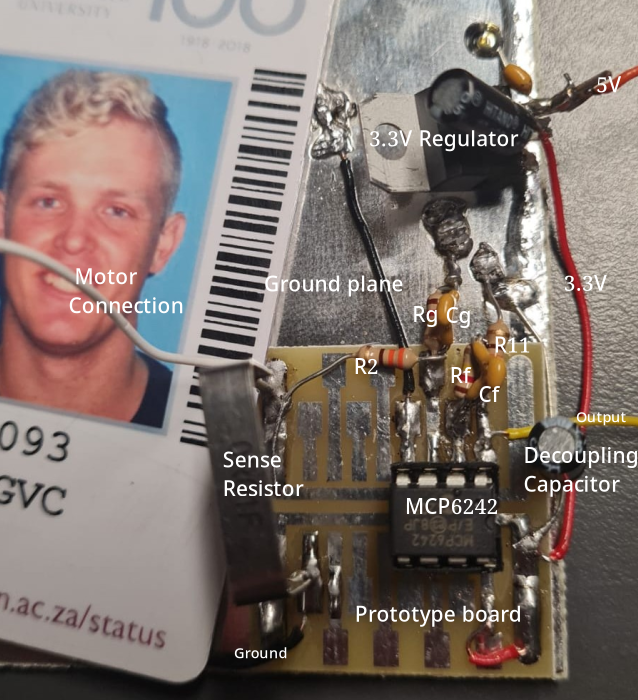
\includegraphics[width=0.75\textwidth]{Figures/physical_circuit}
  \caption{Final Circuit Implementation}
\end{figure}
\include{Chapter5}
\include{Chapter6}


% Bibliography
\bibliography{References}

% End matter
\appendix
\chapter{Social contract}
\makeatletter\@mkboth{}{Appendix}\makeatother
\label{appen:social_contract}
\textcolor{red}{Download copy from SUNLearn, sign and include here (replace this one).}
     \begin{figure}[!htb]
     \centering
     	\fbox{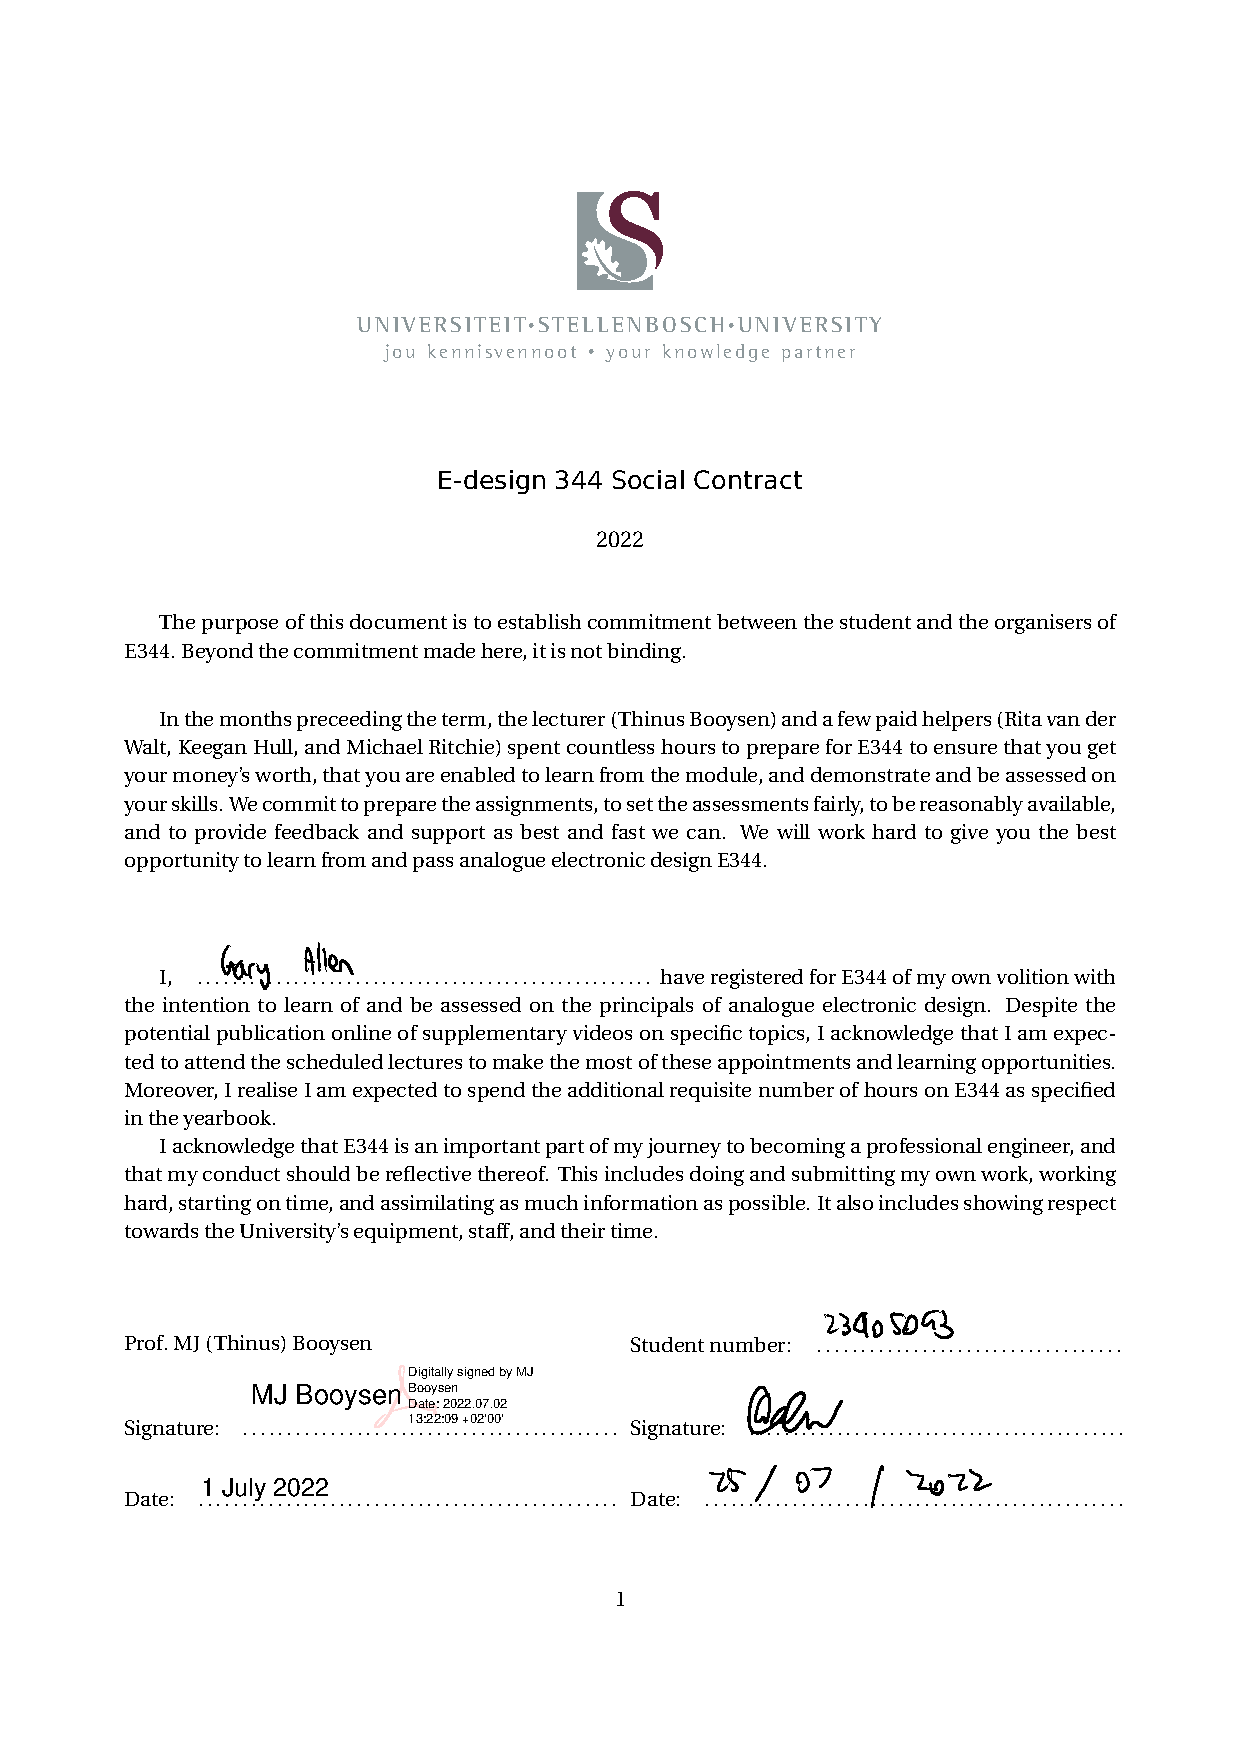
\includegraphics[width=0.8\linewidth]{./Figures/SocialContract_signed.pdf}}
       \label{fig:social_contract}
	\end{figure}
\chapter{GitHub Activity Heatmap}
\makeatletter\@mkboth{}{Appendix}\makeatother
\label{appen:github_heatmap}
\textcolor{red}{Take a screenshot of your github version control activity heatmap and insert here. }

     \begin{figure}[!htb]
     \centering
     	\fbox{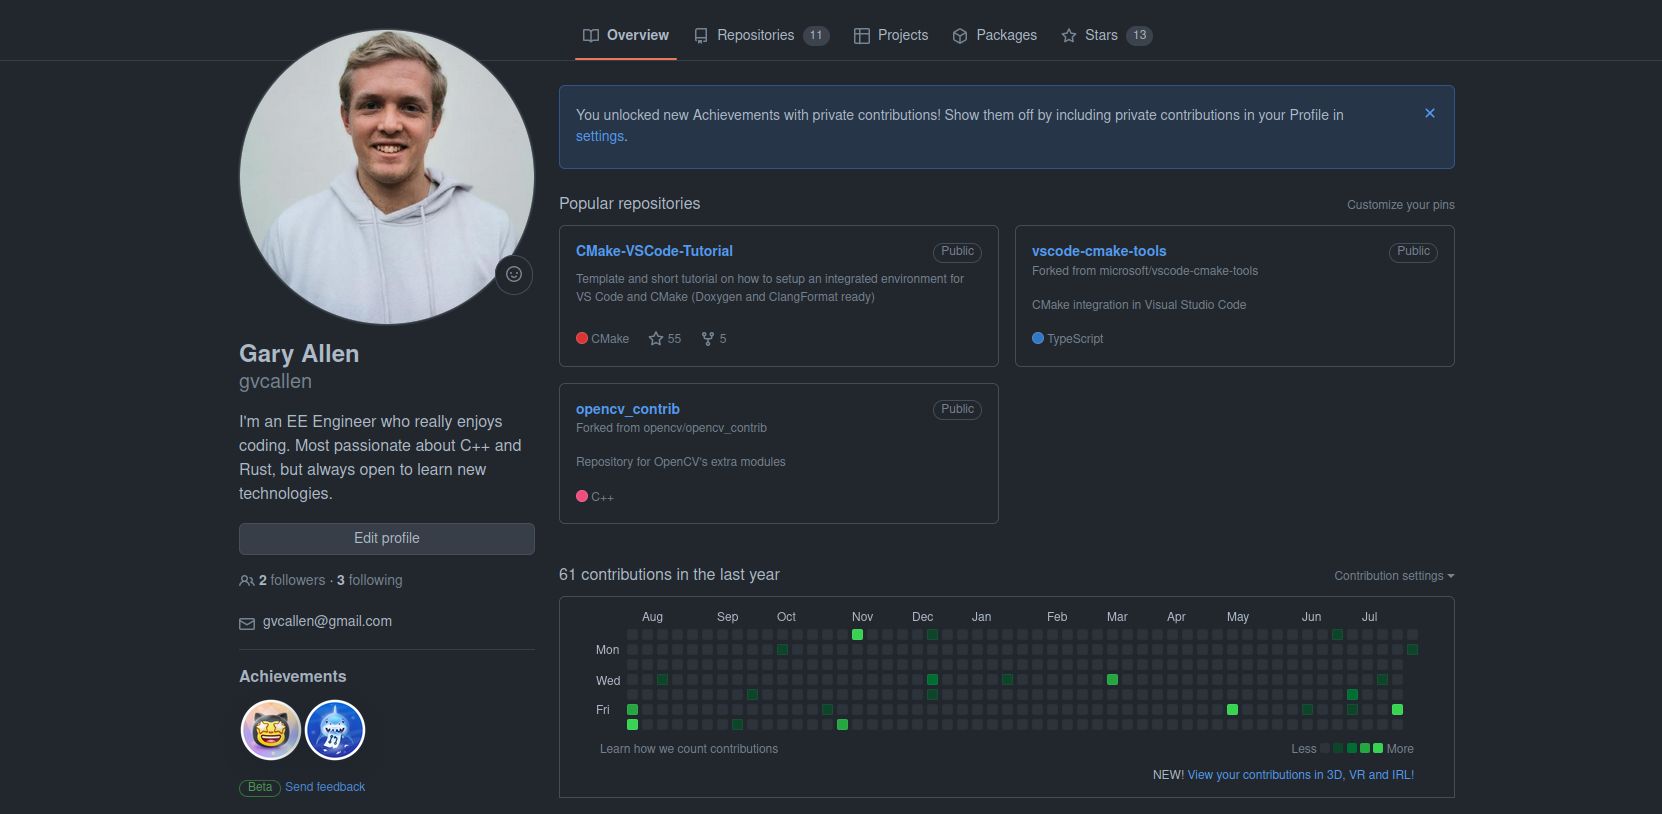
\includegraphics[width=1\linewidth]{./Figures/GitHub.png}}
	\label{fig:github}
	\end{figure}
%\chapter{Stuff you want to include}

\textcolor{red}{remove this if not needed!! \\} 

\textcolor{red}{You can remove this chapter by deleting the ``\texttt{\textbackslash include\{App-C \}}'' line in the \texttt{e344\_A1\_report.tex} file.  }

\lipsum


\end{document}

